\documentclass{article}
\usepackage{tikz}

\begin{document}

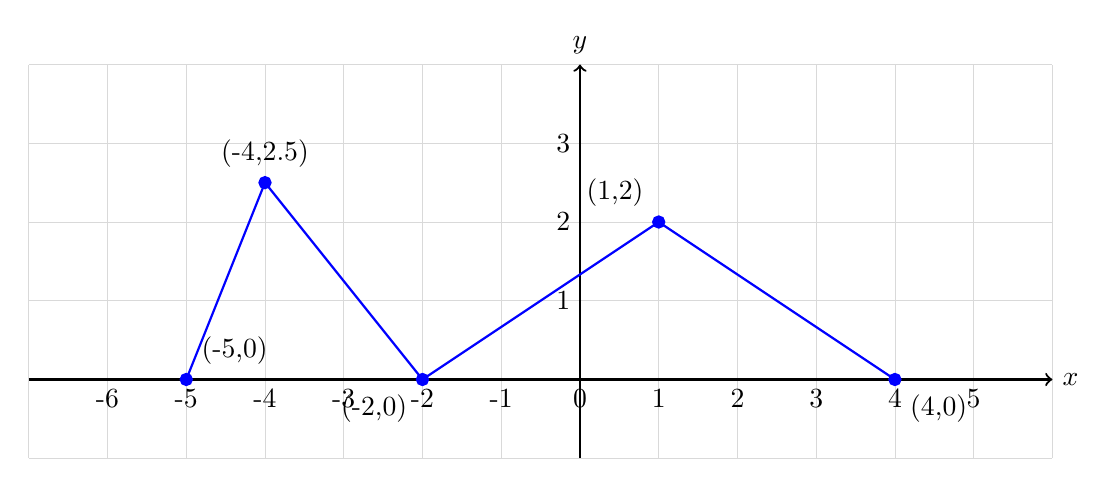
\begin{tikzpicture}[scale=1]
    \draw[gray!30, very thin] (-7,-1) grid (6,4);
    \draw[thick,->] (-7,0) -- (6,0) node[right] {$x$};
    \draw[thick,->] (0,-1) -- (0,4) node[above] {$y$};
    
    % x and y axis labels
    \foreach \x in {-6, -5, ..., 5} {
        \node[anchor=north] at (\x,0) {\x};
    }
    \foreach \y in {1, 2, 3} {
        \node[anchor=east] at (0,\y) {\y};
    }

    % Plotting the points
    \draw[blue, thick, mark=*, mark options={fill=blue}] plot coordinates {
        (-5,0)
        (-4, 2.5)
        (-2, 0)
        (1, 2)
        (4, 0)
    };

    % Annotate the points with some shifts to avoid overlap
    \node[above right, yshift=2pt, xshift=2pt] at (-5,0) {(-5,0)};
    \node[above, yshift=2pt] at (-4,2.5) {(-4,2.5)};
    \node[below left, yshift=-2pt, xshift=-2pt] at (-2,0) {(-2,0)};
    \node[above left, yshift=2pt, xshift=-2pt] at (1,2) {(1,2)};
    \node[below right, yshift=-2pt, xshift=2pt] at (4,0) {(4,0)};
\end{tikzpicture}

\end{document}